\documentclass[12pt,
               a4paper,
               article,
               oneside,
               oldfontcommands,
               norsk]{memoir}
\makeatletter
\newcommand*{\rom}[1]{\expandafter\@slowromancap\romannumeral #1@}
\makeatother
%\usepackage[utf8]{inputenc}
\usepackage{setspace}
\usepackage[T1]{fontenc}
\usepackage{titling}% the wheel somebody else kindly made for us earlier
\usepackage{fancyhdr}
\usepackage{fancybox}
\usepackage{epigraph} 
\usepackage{tikz}
\usepackage{pgfplots}
\pgfplotsset{compat=1.12}
\usepackage{lmodern}
\usepackage{enumitem}
\usepackage{caption}
\usepackage{subcaption}
\usepackage{fancyvrb}
\usepackage[scaled]{beramono}
\usepackage[final]{microtype}
\usepackage{amssymb}
\usepackage{mathtools}
\usepackage{amsthm}
\usepackage{thmtools}
\usepackage{babel}
\usepackage{csquotes}
\usepackage{listings}
\usetikzlibrary{calc,intersections,through,backgrounds}
\usepackage{tkz-euclide} 
\lstset{basicstyle = \ttfamily}
\usepackage{float}
\usepackage{textcomp}
\usepackage{siunitx}
\usepackage{xcolor}
\usepackage{graphicx}
\usepackage[colorlinks, allcolors = uiolink]{hyperref}
\usepackage[noabbrev]{cleveref}
\pretolerance = 2000
\tolerance    = 6000
\hbadness     = 6000
\newcounter{probnum}[section]
\newcounter{subprobnum}[probnum] 
\usepackage{dirtytalk}
\usepackage{listings}
\usepackage{xcolor}
\usepackage{caption}
\usepackage[section]{placeins}
\usepackage{varwidth}
\definecolor{uiolink}{HTML}{0B5A9D}
\definecolor{dkgreen}{rgb}{0,0.6,0}
\definecolor{gray}{rgb}{0.5,0.5,0.5}
\definecolor{mauve}{rgb}{0.58,0,0.82}
\lstset{frame=tb,
  language=R,
  aboveskip=3mm,
  belowskip=3mm,
  showstringspaces=false,
  columns=fullflexible,
  basicstyle={\small\ttfamily},
  numbers=none,
  numberstyle=\tiny\color{gray},
  keywordstyle=\color{blue},
  commentstyle=\color{dkgreen},
  stringstyle=\color{mauve},
  breaklines=true,
  breakatwhitespace=true,
  tabsize=3
} 
\usepackage{commath}
\newtheorem{theorem}{Theorem}[section]
\newtheorem{corollary}{Corollary}[theorem]
\newcommand{\Q}{ \qquad \hfill \blacksquare}
\newcommand\myeq{\stackrel{\mathclap{\normalfont{uif}}}{\sim}}
\let\oldref\ref
\renewcommand{\ref}[1]{(\oldref{#1})}
\newtheorem{lemma}[theorem]{Lemma}
\setlength \epigraphwidth {\linewidth}
\setlength \epigraphrule {0pt}
\AtBeginDocument{\renewcommand {\epigraphflush}{center}}
\renewcommand {\sourceflush} {center}
\parindent 0ex
\renewcommand{\thesection}{\roman{section}} 
\renewcommand{\thesubsection}{\thesection.\roman{subsection}}
\pretitle{
	\begin{center}
		\rule[0.4pt]{300pt}{1.5pt} \\
			[0.10in]
\Huge}
		\title{I Euclids trekantete hage}
\posttitle{\par\vskip0.3em{\scshape \textsc{ \large Prosjektoppgave \\ MAT2500}\\[-0.20in] \rule[0.4pt]{300pt}{1.5pt} \vspace{5mm}}
	\end{center}}
\author{Jonas Semprini Næss}

\begin{document}
\maketitle
\epigraph{\centering Euclid's manner of exposition, progressing relentlessly from the data to the unknown and from the hypothesis to the conclusion, is perfect for checking the argument in detail but far from being perfect for making understandable the main line of the argument.}{\textit{- George Pólya}}
\subsection*{\protect \centering Innledning}
\emph{I det som kan bli sett på som en av matematikkens største tryllekunster (Euclids Elementer), finner vi et hav av geometriske godbiter. Blant disse bølgene av skolerte setninger, teoremer, forslag (\say{Propositions}) og postulater reises det en dyp fasinasjon for de mest fundamentale geometriske strukturer. Det er dermed ingen overraskelse at temaet i dette dykket skal handle om trekanter og noen av dets egenskaper. Vi skal fra starten følge Setning 19 i bind 1, som i sin enkelhet gir utspring til rike og allsidige matematiske faktum, samt forbindelser til kjente resultater i både skole og videregående matematikk.}
\section*{\protect \centering Euclids Elementer}
Euclids elementer på hele tretten bind har siden sin nedtegnelse både formet og revolusjonert geometrien slik vi kjenner den i dag. Fra $300$ f.Kr til den Victorianske perioden var Elementer undervist og benyttet som lærerbok i store deler av Europa. Altså var ikke Elementer kun rigid nok til å tilpasse seg århundrer med matematisk utvikling, men også relevant og godt nok skrevet i en periode uten regnesymboler (jmf. $+, -, \times, \ldots$) og det hindu-arabiske tallsystemet. Hva er det således som gjør Elementer såpass uforanderlig og urørlig?
\section{\large Oppbygning og struktur}
Noe av det som gjør Elementer så merkverdig er hvordan det allerede i bind 1 forekommer 23 definisjoner, 5 postulater, 48 setninger (\say{Propositions}) og 5 allmene slutningsregler (\say{common notions} på engelsk). Dette viser ikke bare hvor heldekkende bind 1 alene er for mye av geometrien vi kjenner til, men også hvor mektig det er som forskningslitteratur i henhold til sin tid. De nevnte posulatene har i sin ettertid vært såpass essensielle at de må nevnes i enhver tekst omhandlende geometri 
\begin{enumerate}
\item Mellom to punkter kan det trekkes en entydig linje.
\item En linje kan forlenges vilkårlig i hver retning.
\item Rundt hvert punkt kan beskrives en sirkel med en vilkårlig radius.
\item Alle rette vinkler er like store.
\item Hvis en rett linje skjærer to rette linjer slik at summen av de indre vinklene på samme side er mindre enn to rette vinkler, da skjærer de to rette linjene hverandre på den siden hvor de indre vinklene befinner seg, når linjene forlenges vilkårlig langt.
\end{enumerate}
hvor attpåtil definisjonene om at et punkt er noe udelelig og linjen er en lengde uten bredde ei kan utestå. Herfra har Euclid konstruert grunnlaget for sin matematikk, som gir ytterligere tyngde i sine geomteriske setninger og observasjoner. I en videre analyse av Euclids setninger (\say{Propositions}) kan det skimtes av Euclid foretar seg to måter å bevise forslagene sine. Den ene er via Q.E.D som svarer til metoden å \say{Bevise det som skulle vises}, og Q.E.F som samsvarer til metoden om å (\say{Bevise det som skulle gjøres}). Ved første øyekast virker disse metodene tilsynelatende veldig like, hvilket de delvis er, men den som store forskjellen er at ved metdoen Q.E.F ligger hovedvekten i den tekniske utførelsen av det geometriske utsagnet/forslaget. Dermed er det en mer konstrukjsonsmessig analyse i metoden fremfor et strigent algebraisk rammeverk (eksempelvis \say{Proposition} 1 i Elementer). \cite{Elementer}
\begin{figure}[H]
\centering
\captionsetup{justification=centering,margin=2cm}
 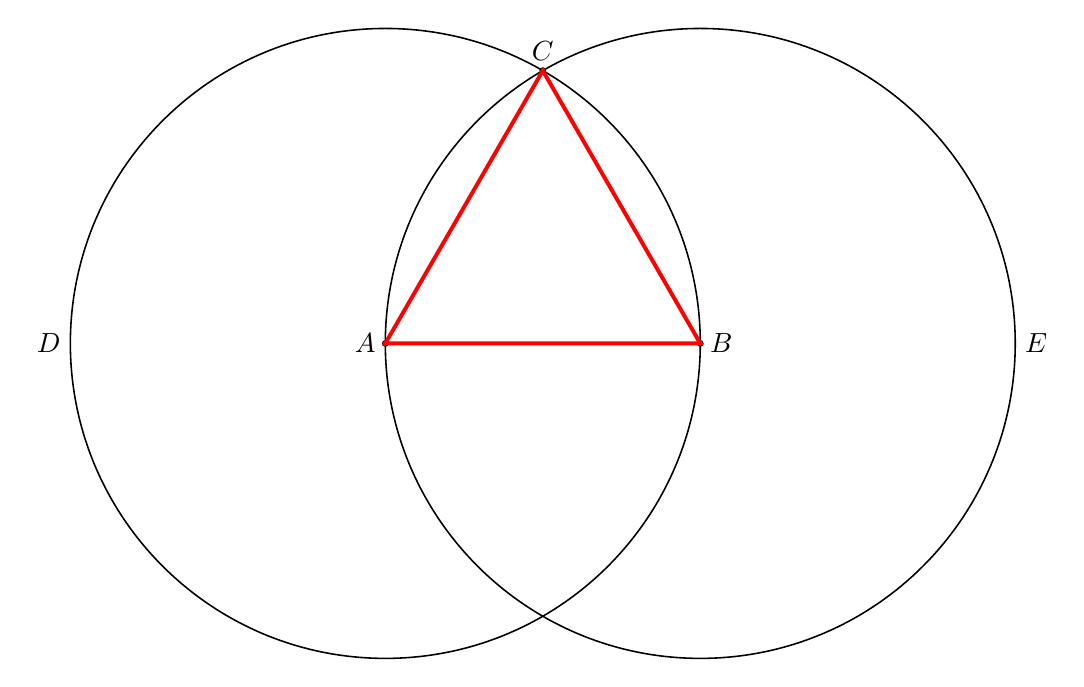
\begin{tikzpicture}[label distance=5mm]
        \tkzDefPoint(0,0){A}
        \tkzLabelPoint[black,anchor=east](A){$A$} 
        \tkzDefPoint(4,0){B}
        \tkzLabelPoint[black,anchor=west](B){$B$}
        \tkzDefPoint(8,0){E}
        \tkzLabelPoint[black,anchor=west](E){$E$} 
        \tkzDefPoint(-4,0){D}
        \tkzLabelPoint[black,anchor=east](D){$D$}
         \draw[name path=circle1, line width=0.2mm, black] (0,0) circle (4cm);
         \draw[name path=circle2, line width=0.2mm, black] (4,0) circle (4cm);
         \tkzInterCC[R](A,4cm)(B,4 cm) \tkzGetPoints{M1}{N1}
         \tkzLabelPoint[black,anchor=south](M1){$C$}
         \tkzDrawPoints(M1)
         \tkzDrawPoints(A)
         \tkzDrawPoints(B)
         \draw[line width=0.5mm, red](A) -- (M1) -- (B) -- cycle;
 \end{tikzpicture}
\caption*{Illustrasjon av setning 1.1 fra Euclids elementer: \vspace{2mm}\\ \emph{To construct an equilateral triangle on a given finite straight line.}}
\end{figure}
\section*{\protect\centering Starten på en trenkantet reise}
En merkbar trend i de 48 setningene i første bind av Elementer er at majoriteten omhandler resultater tilknyttet trekanter. Hvorfor det? Vel, mye ligger nok i at vilkårlige polygoner (mye studert i de senere bindene) kan dekomponeres til trekanter og at tre unike punkter (som er i generell posisjon) definerer en sirkel. Med det sagt var også Euclid vel kjent med mange av resultatene til Pytagoreerne i forbindelse med trekanter. Derfor skal vi nå i Euclids ettermæle studere hva de gamle grekerene funderte over på den skinnende marmoren i sommersolen. 
\section{\large Setning 19 bind 1}
\vspace{4mm}
\shadowbox{\small \emph{I en vilkårlig trekant er den motsatte side av den største vinkel, den største.}} \vspace{3mm} \\ 
Lyder Euclids nittende uttalelse i første bind. Setningen i seg er så enkel som man får det, og med tanke på dagens forståelse av matematikk er det nesten underforstått at dette er sant, men det er som alltid noe litt mer magisk bak skissene her også. For mange lyser nok trigonometripæren opp umiddelbart som vi om litt skal se er en veldig rimelig avgjørelse, men før vi begynner å løpe av sted skal vi se på Euclids metode for å løse problemstillingen. \vspace{4mm}\\
For Euclid var beviset av påstanden noe vanskeligere enn de vi i dag ville antatt, mye til grunn for at hverken algebra var godt nok utviklet ei et trigonometrisk system. Dermed er beviset mer visuelt enn hva et mer moderne bevis ville vært. 
\begin{proof}
  La $\triangle ABC$ være trekanten med $\angle ABC = \alpha$ og $\angle BCA = \beta$ hvor $ \alpha > \beta$.
  \begin{figure}[H]
    \centering 
    % \documentclass[12pt,
%                a4paper,
%                article,
%                oneside,
%                oldfontcommands,
%                norsk]{memoir}
% \usepackage{tikz}
% \usepackage{tkz-euclide}
% \usetikzlibrary{calc,patterns,angles,quotes}
% \begin{document}
\begin{tikzpicture}[label distance=5mm]
    \tkzDefPoint(0,0){C}
    \tkzLabelPoint[black,anchor=north](C){$C$} 
    \tkzDefPoint(4,3){A}
    \tkzLabelPoint[black,anchor=west](A){$A$};
    \tkzDefPoint(1,3){B}
    \tkzLabelPoint[black,anchor=east](B){$B$};
    \draw (A) -- (B) -- (C) -- cycle;
    \tkzMarkAngle[red, size=0.5,mark=None](C,B,A)
    \tkzMarkAngle[blue, size=0.5,mark=None](A,C,B)
    \tkzLabelAngle[pos = .8](C,B,A){$\alpha$}
    \tkzLabelAngle[pos = .9](A,C,B){$\beta$}
\end{tikzpicture}
% \end{document}
    \caption{}
  \end{figure}
Anta så at $\overline{AC} > \overline{AB}$, hvis ikke er $\overline{AC} \leq \overline{AB}$. Men $\overline{AC} \neq \overline{AB}$ siden da ville $\angle ABC = \angle ACB$ ei kan $\overline{AC} < \overline{AB}$ siden da vil  $\angle ABC < \angle ACB$. Således har vi vist at $\overline{AC}$ hverken kan være lik eller mindre enn $\overline{AB}$ som betyr at $\overline{AC}$ må være større enn $\overline{AB}$.
\end{proof} \cite{Prop_19}
Beviset er elegant, kort og konsist. Det mest merkverdige er dog at han benytter seg av en bevismetode som går ut på å oppnå en selvmotsigelse (forekommer flere ganger i Elementer) som vi i dag kjenner til som en av de mest brukte bevisformene; \emph{\textbf{Reductio Ad Absurdum}}. Kjernen i bevisformen er at den appelerer direkte til logikk (enten er det sant eller ikke) som gir markant styrke i en matematisk sammenheng. \vspace{4mm}\\ 
\textbf{\large Sinussetning:} \vspace{2mm}\\ 
Selv om det forekommer geomteriske observasjoner som benyttes i trigonometri i Elementer, er ikke trigonometri selv med. Trigonometri gjør sin opptreden blant senere greske matematikere hvor relasjonen mellom korden på en sirkel og sinus er essensiell. Dermed er det naturlig å se på hvilken effekt trigonometri kan gi når vi analyserer slike problemer. Hvis vi husker tilbake til skolematematikken er sinussetningen definert ved 
\begin{align*}
  \frac{\sin A}{a} =  \frac{\sin B}{b} =  \frac{\sin C}{c} 
\end{align*} 
hvor $a, b, c$ svarer til lengden på motstående sider av de respektive vinklene $A, B, C$.
\begin{figure}[H]
  \centering 
  % \documentclass[12pt,
%                a4paper,
%                article,
%                oneside,
%                oldfontcommands,
%                norsk]{memoir}
% \usepackage{tikz}
% \usepackage{tkz-euclide}
% \usetikzlibrary{calc,patterns,angles,quotes}
% \begin{document}
\begin{tikzpicture}[label distance=5mm]
    \tkzDefPoint(0,0){C}
    \tkzLabelPoint[black,anchor=east](C){$C$} 
    \tkzDefPoint(4,0){A}
    \tkzLabelPoint[black,anchor=west](A){$A$};
    \tkzDefPoint(1,3){B}
    \tkzLabelPoint[black,anchor=south](B){$B$};
    \draw (A) -- (B) node[midway, right] {$c$} -- (C) node[midway, left] {$a$} -- cycle node[midway, below] {$b$};
\end{tikzpicture}
%\end{document}
  \caption{Illustrasjon av sinussetningen.}
\end{figure}
Med andre ord er sinusen til en vinkel i en vilkårlig trekant proposjonal med størrelsen av den motstående side. Da går det kanskje opp et lys at dette er nøyaktig det som trengs for å bevise setning 19 bind 1 i elementer. Hvilket fra illustrasjonen i beviset til Euclid gir
\begin{align*}
\frac{\sin B}{b} = \frac{\sin C}{c} \iff \frac{b}{c} = \frac{\sin B}{\sin C}  
\end{align*}
og 
\begin{align*}
 B &= \arcsin \left( \frac{b}{c} \sin C\right) \\[5pt]
 C &= \arcsin \left( \frac{c}{b} \sin B\right) \\[5pt]
\end{align*}
hvor $\frac{b}{c} > 1$ siden $b > c$ og $B > C$ siden $\left( \frac{b}{c} \sin C\right) > \left( \frac{c}{b} \sin B\right)$ for $0 < B,C < 1$. Sistnevnte kan ses enklere ved å se på $\arcsin(x)$ funksjonen for $x \in [0, 1]$.
\begin{figure}[H]
\centering
\title*{$\arcsin(x), \ x \in [0, 1]$}
% \documentclass[12pt,
%                a4paper,
%                article,
%                oneside,
%                oldfontcommands,
%                norsk]{memoir}
% \usepackage{tikz}
% \usepackage{tkz-euclide}
% \usepackage{pgfplots}
% \pgfplotsset{compat=1.12}
% \usetikzlibrary{calc,patterns,angles,quotes}
% \begin{document}
\begin{tikzpicture}[label distance=5mm]
    \begin{axis}[domain=0:1, samples=500, axis lines*=middle, xtick={0,0.5, 1}, ytick={0.785, 1.57}, yticklabels={$\pi$/4,$\pi$/2}]
        \addplot[color = red]  {asin(x)/180*pi};
        \draw[dashed, blue](0, 0.785) -- (0.70, 0.785);
        \draw[dashed,blue] (0, 1.57) -- (1, 1.57);
        \end{axis}
\end{tikzpicture}
% \end{document}
\end{figure}
Euclid har dermed ikke bare underbygd geometeriens ryggrad, men likeså mye av trigonometrien. En bør dessuten gjøres bemerksom på at selv om resultatet er gjort i utgangspunkt av Figur 1 så gjelder dette for alle vilkårlige trekanter. 
\section{\large Setning 20 bind 1}
\shadowbox{\parbox{\textwidth}{\small\emph{I en vilkårlig trekant er summen av to tilfeldig valgte sider større enn den gjenværende}}}\vspace{3mm}\\ 
Likeså som setning 19 er setning 20 både kort og konsis i sin språkdrakt. Utsagnet virker tilsynelatende likt både i form og informasjon, men har sine forskjeller især av anvendelsesområde. Euclid var som mange spesielt interesserte på sin tid notorisk opptatt av at sine oppdagelser hadde håndfast praktisk tyngde, hvilket kommer ekstra tydelig frem i denne setningen. Ikke bare røpet den viktige egenskaper ved størrelser på en trekant, men også i generelle trekk hvordan en lettere kan avgjøre avstand mellom punkter og hva deres korteste vei er. \vspace{4mm}\\ 
Det ringer nok en bjelle for mange når det nevnes at \say{Den korteste vei mellom to punkter er den rette linje}, og høvelig så. Men hva har det med setning 20 å gjøre? Det nevnes i uttalesen at summen av størrelsene til to vilkårlige sider alltid er større en den gjenværende. Direkte peker dette på at det er en sammenheng mellom avstanden fra ett punkt til et annet samt avstanden til de samme punktene gjennom ett annet. I det følgende beviset skal vi se på hvorfor dette har betyding 
\begin{proof}
  La $\triangle ABC$ hvor vi antar at summen av to vilkårlige sider er større enn den gjenværende, altså, 
\begin{align*}
\overline{BA} + \overline{AC} > \overline{BC}\\[5pt] 
\overline{AB} + \overline{BC} > \overline{AC} \\[5pt] 
\overline{BC} + \overline{CA} > \overline{AB}.
\end{align*}
\begin{figure}[H]
\centering 
% \documentclass[12pt,
%                a4paper,
%                article,
%                oneside,
%                oldfontcommands,
%                norsk]{memoir}
% \usepackage{tikz}
% \usepackage{tkz-euclide}
% \usetikzlibrary{calc,patterns,angles,quotes}
% \begin{document}
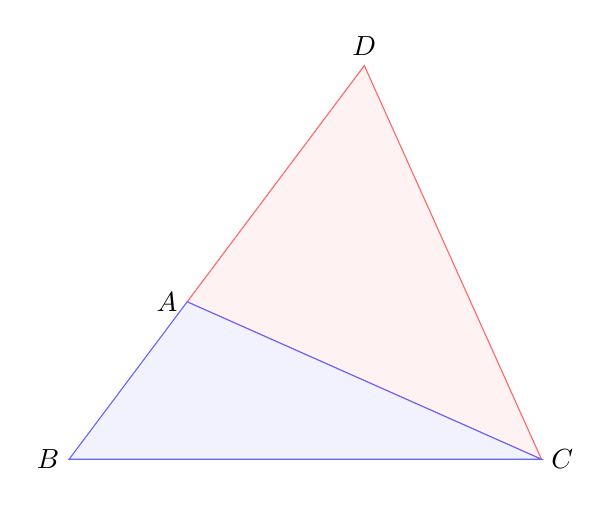
\begin{tikzpicture}[label distance=5mm]
    \tkzDefPoint(0,0){B}
    \tkzLabelPoint[black,anchor=east](B){$B$} 
    \tkzDefPoint(1.5,2){A}
    \tkzLabelPoint[black,anchor=east](A){$A$};
    \tkzDefPoint(6,0){C}
    \tkzLabelPoint[black,anchor=west](C){$C$};
    \tkzDefPoint(3.75,5){D}
    \tkzLabelPoint[black,anchor=south](D){$D$};
    \filldraw[color=red!60, fill=red!5](A) -- (D) -- (C) -- cycle;
    \filldraw[color=blue!60, fill=blue!5](A) -- (B) -- (C) -- cycle;
\end{tikzpicture}
% \end{document}
\caption{Skisse til setning 20}
\end{figure}
Tegn $BA$ gjennom punktet $D$ og sett $\overline{DA} = \overline{CA}$. Slå så sammen $DC$. Siden $DC = AC$ er følgelig $\angle ADC = \angle ACD$ og $\angle BCD > \angle ADC$. Siden $DCB$ er en trekant med $\angle BCD > \angle BDC$ er følgelig den motstående side for $\angle BCD$ størst, nemlig $DB > BC$ (jmf. Setning 19). \vspace{3mm}\\
Men $\overline{DA} = \overline{AC}$ så summen av $BA$ og $AC$ må være større enn $BC$. Lignende kan vi bevise at summen av $AB$ og $BC$ er større enn $CA$ og summmen av $BC$ og $CA$ er større enn $AB$. Derfor må det i enhver trekant være slik at summen av to vilkårlige sider alltid er større enn den gjenværende.
\end{proof}\cite{Prop_20}
\subsection{\large Trekantulikheten:}
Resultatet av setning 20 er i dag bedre kjent som \say{trekantulikheten}. Det er en underforstått del av trekantulikheten at den korteste vei mellom to punkter er den rette linje, og med setning 20 kan en bevise at dette stemmer selv med utgangspunkt i alle mulige polygone stier mellom to punkter. Det er dog også flere tenklige stier enn polygone. \vspace{4mm}\\ 
Trekantulikheten benyttes ikke bare innen geometri, men i mange felt som Reel analyse, Lineær Algebra og Abstrakt Algebra. Spesielt i reel analyse er trekantulikheten grobunn for å definere det som heter metriske rom. Uten å gå for mye inn på hva metriske rom er kan vi forstå metrikken som en funksjon som beregner avstanden mellom to elementer i den mengden metrikken tilhører. Siden metrikken da er en avstandsberegnende funksjon kan vi videreføre dette til å bevise trekantulikheten for generelle metriske rom. \cite{t_ineq}
\begin{proof}
  Anta at vi har elementer $x, y \in X$ hvor $x, y \in \mathbb{R}$. Metrikken på $X$ er dermed gitt ved 
\begin{align*}
d: X \times X \rightarrow \mathbb{R}
\end{align*}
slik at det følgende holder 
\begin{itemize}
  \item $d(x,y) = 0 \iff x = y$ 
  \item $d(x,y) = d(y,x)$
  \item $d(x,z) \leq d(x,y) + d(y,z)$
\end{itemize}
for $x,y,z \in X$. Således kan vi uten tap av generalitet anta fire følgende tilfeller
\begin{enumerate}
  \item $x, y = 0 \ \lor y,z = 0 \ \lor x,z = 0$ 
  \item $x < z, \ x > y$
  \item $x < z, \ y > x$
  \item $x < z, \ z > y$
\end{enumerate}\vspace{3mm}
\textbf{Tilfelle 1:} \vspace{3mm}\\ 
Det er lett å se at hvis to av $x,y,z$ er like så vil eksempelvis $d(x,z) = d(x,y) + d(y,z)$ \vspace{3mm}\\ 
\textbf{Tilfelle 2:}\vspace{3mm}\\ 
La oss anta at $y < x < z$  dermed er $d(x, z) < d(y,z)$ som betyr at vi får $d(x,z) < d(x,y) + d(y,z)$ \vspace{3mm}\\ 
\textbf{Tilfelle 3:}\vspace{3mm}\\
La oss anta at $x < y < z$ da har vi som i tilfelle 1 likhet slik at $d(x,z) = d(x,y) + d(y,z)$. \vspace{3mm}\\ 
\textbf{Tilfelle 4:}\vspace{3mm}\\ 
La oss anta at $x < z < y$ dermed er $d(x,z) < d(x,y$) som gir $d(x,z) < d(x,y) + d(y,z)$. \vspace{4mm}\\ 
Med andre ord vil likhet i trekantulikheten kun eksistere hvis og bare hvis $y$ ligger i mellom $x$ og $z$ eller vi har et tilfelle av tilfelle 1.
\end{proof}
Nok en gang har vi, med utgangspunkt i et primitivt geometrisk utsagn, klart å trekke linjer mellom det Euclid beviste for 2200 år tilbake for vilkårlige trekanter til å gjelde i moderne grener av matematikk som reel analyse. Dessuten er det en bemerkelsesverdig kompletthet i Euclids observasjoner grunnet forenligheten mellom trekanters sider, korteste avstand mellom to gitte punkter samt relasjonen mellom reele tall (jmf beviset av trekanulikheten ovenfor). Som ganske enkelt viser hvor tilknyttet geometri er til alle aspekter av matematikk. 
\section{Setning 24 bind 1}
\shadowbox{%
\parbox{\textwidth}{\small\emph{Hvis to vilkårlige trekanter har to respektive like sider, men hvorav vinkelen inneholdt mellom disse linjene i en av trekantene er større, vil den således ha større grunnlinje}}}\vspace{4mm}\\ 
Slutten på den trekantente reise av Elementer ender på setning 24 i bind 1. Symmetriske og proposjonale egenskaper er et gjennomgående tema både i de setningene vi har sett på, men også i majoriteten av bindene i Elementer. Derfor er det høvelig å avslutte med en observasjon som er likeså. Formuleringen av setningen virker noe kronglete ut i fra hva som skal vises, men ved litt nærmere undersøkelse så deler den i store trekk nettopp det setning 19 innbefatter. \vspace{4mm}\\ 
\begin{proof}
La $\triangle ABC$ og $\triangle DEF$ være slik at $AB = AC$ og $DE = DF$ respektivt. Dette betyr videre fra antagelsen at $AB = DE$ og $AC = DE$. La så $\angle BAC > \angle EDF$, hvor jeg påstar at $BC > EF$.
\begin{figure}[H]
  \centering
  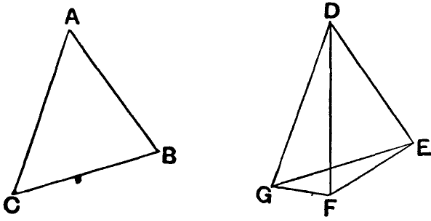
\includegraphics[scale=2.8]{setning_24.png}
  \caption{Trekanter $\triangle ABC, \ \triangle DEF$}
\end{figure}
Siden $\angle BAC > \angle EDF$, kan en konstruere vinkelen $\angle EDG$ lik $\angle BAC$ i punktet $D$ på den rette linje $DE$. La så $DG$ være lik enten $AC$ eller $DF$ og slå sammen $EG$ og $EF$. \vspace{2mm}\\ 
Siden $AB = DE$ og $AC = DG$, er $BA$ og $AC$ lik de to respektive sidene $ED$ og $DG$ og $\angle BAC = \angle EDG$, hvilket betyr at grunnlinjene $BC = EG$. \vspace{4mm}\\
Igjen, siden $DF = DG$ er følgelig $\angle DGF = \angle DFG$. Dermed er $\angle DFG > \angle EFG$ og $\angle EFG >> \angle EGF$. \vspace{4mm}\\ 
Siden $\triangle EFG$ er en trekant hvor vinkel $EFG$ er større enn $EGF$ vil siden ovenfor den største vinkel være den største (Setning 19) som betyr at $EG > EF$. Men $EG = BC$ og dermed er også $BG > EF$. \vspace{4mm}\\ 
Dermed kan vi konkludere med at \emph{hvis to vilkårlige trekanter har to respektive like sider, men hvorav vinkelen inneholdt mellom disse linjene i en av trekantene er større, vil den således ha større grunnlinje}.
\end{proof}\cite{Prop_24}\vspace{4mm}
Ikke bare er setningen ett greit verktøy å benytte seg av når man skal se på proposjonalitet blant trekanter, men det er også særlig behjelpelig hvis man ønsker å konstruere trekanter med større areal som likevel bevarer samme form og fasong som en annen. Derfor var det både elegant og passelig å avslutte (i regi av Euclid) med et mer konstrukjsonsmessig preget bevis.

\section*{\centering Oppsummering}
Euclid og hans elementer var og er det mest gjennomførte og heldekkende matematikken har vært borte i. Bredden i innhold suppelert med bevis, konstruksjoner og tankemåter for å forstå komplekse sider ved geometrien har selv med tiden vist seg å være såpass rigid at det til den oppgaven i dag (og til alle tider fremover) vil være et verk å ta nytte av. Hans dype fascinasjon for geomtriske objekter skinner tvers igjennom i alle bind og selv om vi kun fikk besøkt en liten smule fra skattekisten så stopper ikke magien der. De enkle setningene fra bind 1 har vært med på å forme vår forståelse av trekanter og ikke minst det vi kan om trigonometri, dessuten hadde ei geomterien vært like spennende. Euclid har vært med på å forme den moderne matematikken, og i hans arv skal vi likeså videreføre den.
\begin{thebibliography}{5}
    \bibitem{Elementer} 
    Wikipedia.
    \textit{Elements}. Wikipedia\\
    \url{https://en.wikipedia.org/wiki/Euclid%27s_Elements} (lastet ned 23.10.2021, sist oppdatert: 25 October 2021, at 13:31 (UTC)).
    \bibitem{Prop_19} 
    David E. Joyce. 
    \textit{Proposition 19, Book 1}. David E. Joyce \\
    \url{https://mathcs.clarku.edu/~djoyce/elements/bookI/propI19.html} (lastet ned 24.10.2021).
    
    \bibitem{Prop_20} 
    David E. Joyce.\\
    \textit{Proposition 20, Book 1}. David E. Joyce\\
    \url{https://mathcs.clarku.edu/~djoyce/elements/bookI/propI20.html} (lastet ned 24.10.2021)
    
    \bibitem{Prop_24} 
    David E. Joyce.\\  
    \textit{Proposition 24, Book 1}.
    David E. Joyce\\
    \url{https://mathcs.clarku.edu/~djoyce/elements/bookI/propI24.html} (lastet ned 25.10.2021)
   
    \bibitem{t_ineq} 
    Wikipedia.\\  
    \textit{Triangle Inequality}.
    Wikipedia\\
    \url{https://en.wikipedia.org/wiki/Triangle_inequality}(lastet ned 1.11.2021, sist oppdatert:  31 October 2021, at 20:36 (UTC)).

    
    
\end{thebibliography}
\end{document}